%%%%%%%%%%%%%%%%%%%%%%%%%%%%%%%%%%%%%%%%%%%%%%%%%%%%%%%%%%%%%%%%%%%%%%%%%%%%%%%
%                       CARREGA DE LA CLASSE DE DOCUMENT                      %
%                                                                             %
% Les opcions admissibles son:                                                %
%      12pt / 11pt            (cos dels tipus de lletra; no feu servir 10pt)  %
%                                                                             %
% catalan/spanish/english     (llengua principal del treball)                 %
%                                                                             % 
% french/italian/german...    (si necessiteu fer servir alguna altra llengua) %
%                                                                             %
% listoffigures               (El document inclou un Index de figures)        %
% listoftables                (El document inclou un Index de taules)         %
% listofquadres               (El document inclou un Index de quadres)        %
% listofalgorithms            (El document inclou un Index d'algorismes)      %
%                                                                             %
%%%%%%%%%%%%%%%%%%%%%%%%%%%%%%%%%%%%%%%%%%%%%%%%%%%%%%%%%%%%%%%%%%%%%%%%%%%%%%%

\documentclass[11pt,spanish,listoffigures,listoftables]{tfgetsinf}

%%%%%%%%%%%%%%%%%%%%%%%%%%%%%%%%%%%%%%%%%%%%%%%%%%%%%%%%%%%%%%%%%%%%%%%%%%%%%%%
%                     CODIFICACIO DEL FITXER FONT                             %
%                                                                             %
%    windows fa servir normalment 'ansinew'                                   %
%    amb linux es possible que siga 'latin1' o 'latin9'                       %
%    Pero el mes recomanable es fer servir utf8 (unicode 8)                   %
%                                          (si el vostre editor ho permet)    % 
%%%%%%%%%%%%%%%%%%%%%%%%%%%%%%%%%%%%%%%%%%%%%%%%%%%%%%%%%%%%%%%%%%%%%%%%%%%%%%%

\usepackage[utf8]{inputenc} 
\usepackage{multirow}

\usepackage{natbib}
\bibliographystyle{plain}
\graphicspath{ {Imagenes/} }

%%%%%%%%%%%%%%%%%%%%%%%%%%%%%%%%%%%%%%%%%%%%%%%%%%%%%%%%%%%%%%%%%%%%%%%%%%%%%%%
%                        ALTRES PAQUETS I DEFINICIONS                         %
%                                                                             %
% Carregueu aci els paquets que necessiteu i declareu les comandes i entorns  %
%                                          (aquesta seccio pot ser buida)     %
%%%%%%%%%%%%%%%%%%%%%%%%%%%%%%%%%%%%%%%%%%%%%%%%%%%%%%%%%%%%%%%%%%%%%%%%%%%%%%%



%%%%%%%%%%%%%%%%%%%%%%%%%%%%%%%%%%%%%%%%%%%%%%%%%%%%%%%%%%%%%%%%%%%%%%%%%%%%%%%
%                        DADES DEL TREBALL                                    %
%                                                                             %
% titol, alumne, tutor i curs academic                                        %
%%%%%%%%%%%%%%%%%%%%%%%%%%%%%%%%%%%%%%%%%%%%%%%%%%%%%%%%%%%%%%%%%%%%%%%%%%%%%%%

\title{ Desarrollo de software basado en microservicios: un caso de estudio para evaluar sus ventajas e inconvenientes }
\author{Víctor Alberto Iranzo Jiménez}
\tutor{Patricio Orlando Letelier Torres}
\curs{2017-2018}

%%%%%%%%%%%%%%%%%%%%%%%%%%%%%%%%%%%%%%%%%%%%%%%%%%%%%%%%%%%%%%%%%%%%%%%%%%%%%%%
%                     PARAULES CLAU/PALABRAS CLAVE/KEY WORDS                  %
%                                                                             %
% Independentment de la llengua del treball, s'hi han d'incloure              %
% les paraules clau i el resum en els tres idiomes                            %
%%%%%%%%%%%%%%%%%%%%%%%%%%%%%%%%%%%%%%%%%%%%%%%%%%%%%%%%%%%%%%%%%%%%%%%%%%%%%%%

\keywords{Microservices, Arquitecturas de software, ?????????????????} % Paraules clau 
         {Microservicios, Arquitecturas de software, ???????????????}              % Palabras clave
         {Microservices, Software Architecture, ?????????????}        % Key words

%%%%%%%%%%%%%%%%%%%%%%%%%%%%%%%%%%%%%%%%%%%%%%%%%%%%%%%%%%%%%%%%%%%%%%%%%%%%%%%
%                              INICI DEL DOCUMENT                             %
%%%%%%%%%%%%%%%%%%%%%%%%%%%%%%%%%%%%%%%%%%%%%%%%%%%%%%%%%%%%%%%%%%%%%%%%%%%%%%%

\begin{document}

%%%%%%%%%%%%%%%%%%%%%%%%%%%%%%%%%%%%%%%%%%%%%%%%%%%%%%%%%%%%%%%%%%%%%%%%%%%%%%%
%              RESUMS DEL TFG EN VALENCIA, CASTELLA I ANGLES                  %
%%%%%%%%%%%%%%%%%%%%%%%%%%%%%%%%%%%%%%%%%%%%%%%%%%%%%%%%%%%%%%%%%%%%%%%%%%%%%%%

\begin{abstract}
????
\end{abstract}
\begin{abstract}[spanish]
????
\end{abstract}
\begin{abstract}[english]
????
\end{abstract}

%%%%%%%%%%%%%%%%%%%%%%%%%%%%%%%%%%%%%%%%%%%%%%%%%%%%%%%%%%%%%%%%%%%%%%%%%%%%%%%
%                              CONTINGUT DEL TREBALL                          %
%%%%%%%%%%%%%%%%%%%%%%%%%%%%%%%%%%%%%%%%%%%%%%%%%%%%%%%%%%%%%%%%%%%%%%%%%%%%%%%

\mainmatter

%%%%%%%%%%%%%%%%%%%%%%%%%%%%%%%%%%%%%%%%%%%%%%%%%%%%%%%%%%%%%%%%%%%%%%%%%%%%%%%
%                                  INTRODUCCION                                %
%%%%%%%%%%%%%%%%%%%%%%%%%%%%%%%%%%%%%%%%%%%%%%%%%%%%%%%%%%%%%%%%%%%%%%%%%%%%%%%

\chapter{Introducci\'on}

\section{Motivaci\'on}

% Referencia a The Clean Architecture.
En la actualidad, no es necesario un alto grado de conocimientos en ingeniería del software para desarrollar una aplicación o sistema. Personas que no tienen estudios relacionados con la informática pueden producir código que, sin ser limpio y elegante, funciona. Desarrollar sistemas de calidad requiere de grandes conocimientos, pero minimiza los costes y aumenta la productividad de una organización. Se debe poner el foco en emplear una arquitectura de software que se adapte a nuestras necesidades. De lo contrario, el futuro mantenimiento será más costoso y repercutirá en la confianza de los clientes y en la moral del equipo. \cite{Martin2017}

% TODO: Demasiados términos que se deben explicar.
Las arquitecturas basadas en microservicios son una tendencia actual que emerge asociada a conceptos clave como la integración continua, el desarrollo centrado en el dominio del problema o el despliegue en contenedores. En estas arquitecturas diferentes funcionalidades se encapsulan en servicios pequeños y autónomos que cooperan entre ellos. En términos de diseño, principios como el de Responsabilidad Única son más fáciles de conseguir y los desafíos de organización del código pueden abordarse de formas más diversas por la baja granularidad de la arquitectura. 

\section{Objetivos}

El objetivo de este proyecto es validar con un caso de estudio las ventajas e inconvenientes de una arquitectura basada en microservicios frente a una arquitectura monolítica. Concretamente,los objetivos específicos son:

\begin{itemize}

\item Desarrollar una misma aplicación para la venta de productos y la gestión de pedidos siguiendo dos arquitecturas diferentes: una basada en microservicios y otra monolítica.

\item Comparar el proceso de desarrollo de ambos sistemas a lo largo del ciclo de vida del software.

\item Evaluar cómo se pueden llevar a cabo diferentes modificaciones durante el mantenimiento de ambas aplicaciones una vez se ha finalizado su implementación.

\item Verificar que una arquitectura basada en microservicios facilita alcanzar los requisitos no funcionales de escalabilidad y tolerancia a fallos frente a una arquitectura monolítica.

\end{itemize}

\section{Estructura de la memoria}

%%%%%%%%%%%%%%%%%%%%%%%%%%%%%%%%%%%%%%%%%%%%%%%%%%%%%%%%%%%%%%%%%%%%%%%%%%%%%%%
%                                  ESTADO DEL ARTE                                %
%%%%%%%%%%%%%%%%%%%%%%%%%%%%%%%%%%%%%%%%%%%%%%%%%%%%%%%%%%%%%%%%%%%%%%%%%%%%%%%

\chapter{Estado del arte}

\section{¿Qué son los microservicios?}

Según Newman, los microservicios son servicios pequeños y autónomos que trabajan conjuntamente. \cite{Newman2015a} Podemos desglosar esta definición así:

\begin{itemize}
%TODO Sustituir referencia a Wikipedia.

\item Un \textbf{servicio} es un conjunto de funcionalidades que se expone a los clientes para que las empleen con diferentes propósitos. \cite{Wikipedia} La programación orientada a servicios es un paradigma que se aplica en las arquitecturas orientadas a servicios (SOA). El objetivo principal de SOA es desarrollar servicios que aporten valor al negocio y se adapten a los cambios en las necesidades de los clientes, de forma ágil y con el menor coste posible. Las arquitecturas orientadas a servicios no están asociadas a ninguna tecnología específica. En líneas generales, dividen un sistema en componentes que cambian por el mismo motivo y promueven la flexibilidad y los servicios compartidos frente a implementaciones específicas y óptimas. Son muchos los beneficios de estas arquitecturas, sin embargo existe una falta de consenso sobre cómo debe llevarse a cabo este tipo de arquitecturas en aspectos como los protocolos de comunicación a emplear o la granularidad de los servicios. \cite{Arsanjani2009a} Los microservicios pueden entenderse como una aproximación específica de las arquitecturas SOA.

\item Diseñar microservicios con el menor \textbf{tamaño} posible no debe ser el foco principal. En todo momento han de cumplirse los principios de cohesión y coherencia: el código relacionado debe agruparse conjuntamente porque será modificado por el mismo motivo.

\item  Los servicios han de ser lo menos acoplados posibles para garantizar la \textbf{autonomía} de cada uno. Cada microservicio es una entidad separada: cambian de forma independiente al resto y al hacerlo sus consumidores no necesiten ser modificados, a menos que se modifique el contrato entre ambas partes. Para lograrlo, lo más habitual es que cada servicio exponga una interfaz (API) y todas las comunicaciones se realicen mediante llamadas a través de la red.

\end{itemize}

Otra definición interesante es la que aportan Lewis y Fowler. Según ellos, los microservicios son una aproximación para desarrollar una aplicación compuesta por pequeños servicios, cada uno ejecutándose en su propio proceso y comunicando a través de mecanismos ligeros. Estos servicios se construyen alrededor de las capacidades de negocio y se despliegan de forma independiente. \cite{Lewis2014} Cada funcionalidad se encapsula en un servicio que puede escalar de forma diferente de acuerdo a sus necesidades, a diferencia de las aplicaciones monolíticas donde se debe replicar el monolito al completo.

\begin{figure}[h]
\centering
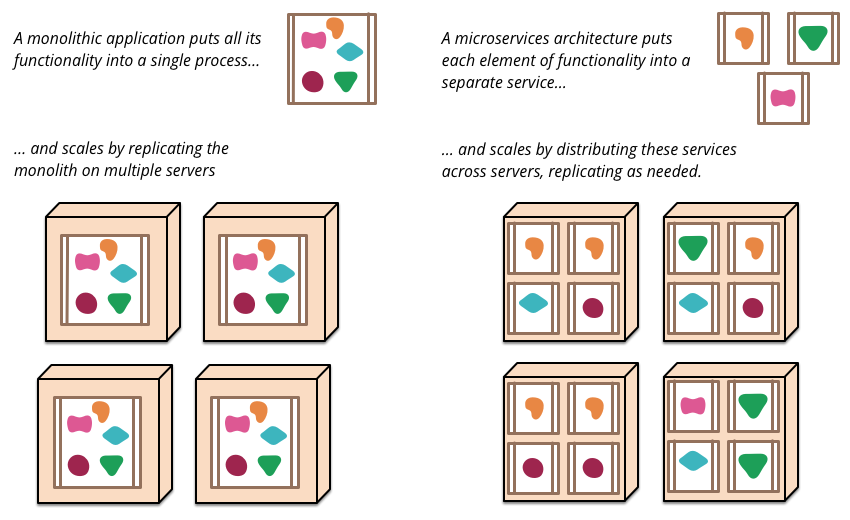
\includegraphics[scale=0.4]{microservices_escaling}
\caption{Los microservicios escalan de acuerdo a su carga de trabajo para asegurar la disponibilidad de la funcionalidad que ofrecen. \cite{Lewis2014}}
\end{figure}

\section{Los microservicios en la fase de requisitos}

La fase de requisitos del software es aquella en la que se elicitan, analizan, documentan, validan y mantienen los requisitos del sistema. Los requisitos del software expresan las necesidades y restricciones asociadas a un sistema. \cite{Fernandes2016} El artefacto principal que se produce en esta fase es el documento con la especificación de requisitos software (ERS). Una vez validado dicho documento por los stakeholders se puede iniciar la fase de diseño la solución. Esto no significa el final de esta fase del proceso: la gestión de los requisitos continúa durante el resto del desarrollo del producto.

\subsection{Requisitos funcionales y no funcionales}

Los requisitos se pueden clasificar en funcionales y no funcionales. Los \textbf{requisitos funcionales} (RF) describen la funcionalidad que los usuarios esperan del sistema. Los \textbf{requisitos no funcionales} (RNF) son restricciones impuestas sobre el sistema a desarrollar, estableciendo por ejemplo como de rápido o fiable ha de ser. Mientras que los primeros no incluyen ninguna mención relacionada con la tecnología que emplea el sistema, los segundos sí pueden establecer restricciones de este tipo. Por ejemplo, un requisito no funcional puede consistir en desarrollar una aplicación en un lenguaje de programación específico o hacer que esté disponible para diferentes sistemas operativos móviles. Por este motivo, los requisitos deben ser tenidos en cuenta a lo largo de todo el desarrollo del sistema.

Los requisitos funcionales y no funcionales son ortogonales en el sentido de que diferentes diseños de software pueden ofrecer la misma funcionalidad (RF) pero con distintos atributos de calidad (RNF). Los arquitectos software están más centrados en los requisitos no funcionales porque estos son los que conducen hacia la elección de una u otra arquitectura. Los requisitos no funcionales pueden influir en los patrones arquitectónicos a seguir, las futuras estrategias de implementación del sistema o la plataforma sobre la que se desplegará el sistema. \cite{Ameller2013}

\begin{figure}[h]
\centering
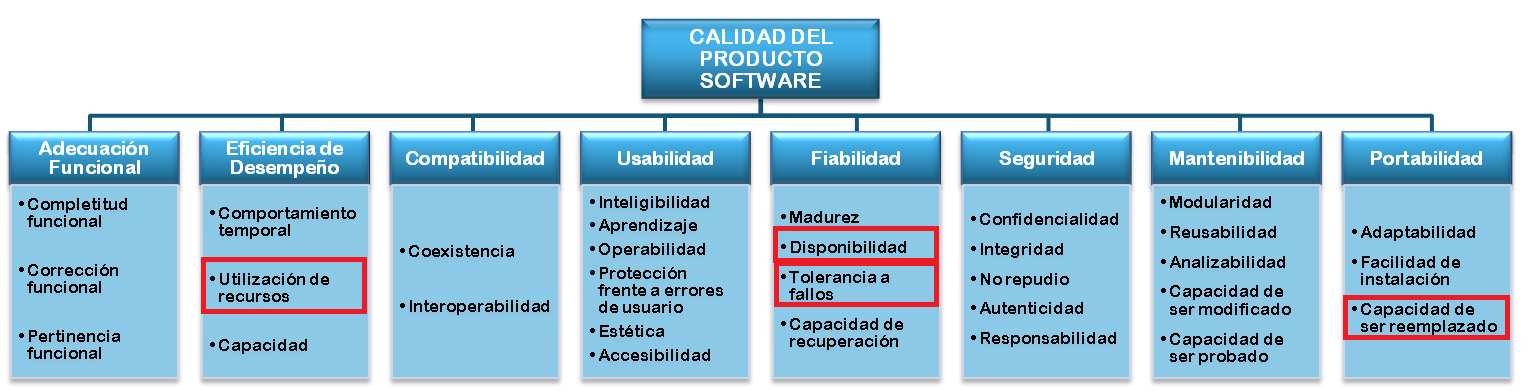
\includegraphics[scale=0.5]{iso25010}
\caption{Características y subcaracterísticas definidas en el modelo de calidad del producto de la ISO/IEC 25010. \cite{Standard2010}}
\end{figure}

Requisitos no funcionales asociados a atributos de calidad como la tolerancia a fallos o la disponibilidad pueden conducir al arquitecto hacia la elección de una arquitectura basada en microservicios:

\begin{itemize}

\item La \textbf{tolerancia a fallos} se define en la ISO/IEC 25010 como la capacidad del sistema para operar según lo previsto en presencia de fallos hardware o software. \cite{Standard2010} Cuando se escala un sistema, la probabilidad de fallo es inevitable. Muchas organizaciones invierten mucho esfuerzo en evitar que un fallo se produzca, pero muy poco en mecanismos para recuperar el sistema una vez se ha producido. Un sistema que por culpa de un servicio caído deja de funcionar es menos resilente que un sistema que puede continuar ofreciendo el resto de sus funcionalidades.

\item La \textbf{disponibilidad} se define como la capacidad del sistema de estar operativo y accesible para su uso cuando se requiere. \cite{Standard2010} En los sistemas distribuidos existen 3 características sobre las que se debe hacer balance: la consistencia, que establece que vamos a obtener una respuesta correcta de cualquier nodo de un servicio de acuerdo a su especificación, la disponibilidad, que ya hemos definido, y la tolerancia a particiones, que es la habilidad de gestionar situaciones en las que la comunicación entre las partes de un sistema se interrumpe. El teorema de CAP (debe sus siglas a las características en inglés Consistency, Availability y Partition Tolerance) establece que en caso de fallo, solo dos de las tres características pueden prevalecer. \cite{Gilbert2012}

\end{itemize}

\subsection{El teorema de CAP}

Pongamos un ejemplo en el que un microservicio está replicado y se produce un fallo por el cual la comunicación entre las replicas se interrumpe y los cambios en una replica no se pueden propagar al resto. Los \textbf{sistemas AP} son los sistemas que surgen fruto de sacrificar la consistencia cuando un fallo se produce, mientras que en los \textbf{sistemas CP} se pierde la disponibilidad. 

En el primer tipo, las replicas continuarían operativas, pero como los datos entre las replicas no se sincronizan se pueden obtener datos incorrectos al hacer una consulta. Cuando la comunicación se restablece, los cambios entre las replicas se sincronizarán. En los sistemas CP, para mantener la consistencia entre las replicas se tiene que rechazar cualquier petición, con lo que el servicio deja de estar disponible.

Los sistemas AP escalan más fácilmente y son más sencillos de construir, pero nos obligan a una consistencia eventual de los datos. Los segundos son los únicos que nos aseguran una consistencia fuerte, pero son más difíciles de construir. A la hora de optar por una solución u otra se debe tener en cuenta la especificación de requisitos, donde se debe detallar de forma específica y cuantitativa cuánto tiempo puede nuestro servicio estar inoperativo o con un dato obsoleto. Si en las fases siguientes se opta por una arquitectura basada en microservicios, no será necesario implementar el sistema completo de una u otra forma. Cada microservicio tendrá necesidades diferentes y podrá seguir la aproximación que mejor le convenga. \cite{Newman2015a}

\section{Los microservicios en la fase de diseño}

En la fase de diseño se definen la arquitectura, componentes e interfaces del sistema. La especificación de requisitos es analizada para producir una descripción de la estructura interna del sistema, con el suficiente nivel de detalle para que sirva como base en su construcción. En esta fase se plantean diferentes diseños como alternativas de las que se debe hacer balance. Los modelos que se generan se emplearán para validar que se cumplen los requisitos establecidos y para planificar la fase de implementación. \cite{Bourque2014}

\subsection{Librerías versus servicios}

Un componente es una unidad de software que se puede reemplazar y actualizar de forma independiente. Las \textbf{librerías} son componentes que están ligados a un programa y son invocadas a través de llamadas a funciones. En cambio, los \textbf{servicios} son componentes que se ejecutan como procesos externos y con los que se puede comunicar a través de mecanismos como llamadas a procedimientos remotos (RPC) o peticiones HTTP. \cite{Lewis2014}

Uno de los motivos por los que se recomienda emplear servicios frente a librerías es que los servicios se pueden desplegar de forma independiente. Solo algunos cambios en la interfaz o contrato del servicio requerirán un cambio en sus consumidores. Además, algunas librerías obligan al uso específico de una tecnología. Sin embargo, las llamadas remotas son más costosas que las invocaciones dentro del mismo proceso, por lo que la interfaz del servicio debe definirse de tal forma que sus consumidores no tengan que comunicarse con él continuamente.

\subsection{Diseño guiado por el dominio (DDD)}

El \textbf{diseño guiado por el dominio} (DDD) es un enfoque para el desarrollo de software que propone un modelado rico, expresivo y evolutivo basado en la realidad del negocio. El dominio representa lo que hace una organización y la forma en qué lo hace.

Con esta aproximación los expertos del dominio y los desarrolladores se sitúan en el mismo nivel empleando un lenguaje ubicuo. No hace falta ninguna traducción de términos entre ellos porque todos hablan un lenguaje común, que se plasma hasta en el código de programación. El lenguaje no tiene porque seguir los estándares de la industria que representa: emplea los términos y acciones que en el negocio se dan. \cite{Vaughn2013}

El lenguaje ubicuo que se emplea crece y cambia con el paso del tiempo. Nadie es capaz de conocer el dominio de un negocio completo porque este forma parte de un proceso de descubrimiento continuo. Si la organización sigue una estrategia de desarrollo ágil, en cada iteración se refina el modelo de forma incremental y este plasma en todo momento el software en funcionamiento.

Para su tratamiento, las áreas independientes del dominio se transforman en contextos delimitados. Cada contexto delimitado es un límite explícito que tiene su propio lenguaje ubicuo. Un concepto tiene un significado dentro de un contexto delimitado, pero fuera de él puede tener un significado totalmente diferente. No se puede tratar de incluir todos los conceptos en un único contexto: se deben separar los conceptos en diferentes contextos y entender las diferencias que existen para un concepto llamado igual en uno y otro contexto.

\begin{figure}[h]
\centering
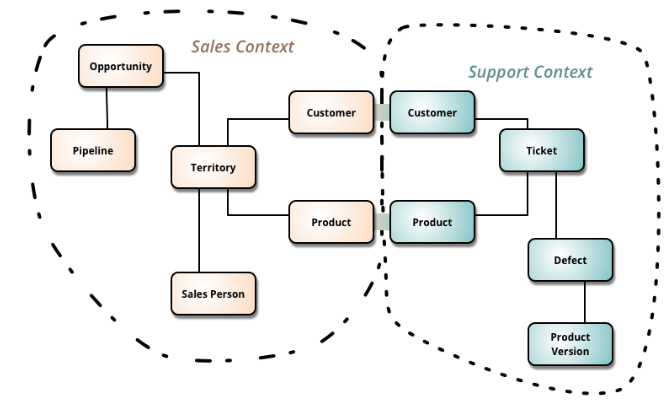
\includegraphics[scale=0.8]{bounded_contexts}
\caption{Ejemplo de dos contextos delimitados dentro del mismo dominio que emplean el mismo nombre para un concepto, pero con significados diferentes. \cite{Fowler}}
\end{figure}

Cada contexto está formado por modelos que no necesitan ser compartidos con otros a menos que se defina explícitamente una interfaz que los empleen. La interfaz es el punto de entrada para que otros contextos puedan comunicar con el nuestro, empleando los términos y entidades que en nuestros modelos se definan.

Esta perspectiva puede trasladarse fácilmente al modelado de microservicios. Los contextos delimitados que analicemos en nuestro sistema son firmes candidatos a transformarse en servicios. Así, los límites de un servicio quedan bien limitados porque  todas las entidades que pueda requerir se encuentran dentro de sus fronteras, garantizándose su alta cohesión y bajo acoplamiento. \cite{Newman2015a}

\subsection{Descomposición en microservicios}

Cuando se razona sobre los límites de un servicio no se debe pensar en los datos que este almacena sino en las funcionalidades que ofrece. Pensar en los datos que almacena nos conduce a desarrollar únicamente servicios CRUD (en inglés, aquellos que nos permiten las operaciones de crear, leer, actualizar y eliminar datos), que ofrecen unas operaciones muy limitadas. Un servicio ofrece ciertas funcionalidades o capacidades que aportan \textbf{valor al negocio}.

Una descomposición temprana de un sistema en microservicios puede conllevar ciertos riesgos. Si el equipo a cargo del desarrollo tiene pocos conocimientos del dominio del problema a resolver, puede  ser buena idea comenzar la implementación como si de un sistema monolítico se tratara. 

Es aconsejable dividir la solución en grandes servicios que poco a poco se vayan dividiendo en más pequeños conforme se estudien las ventajas de hacer cada nueva extracción. Una vez sean conocidos los límites de cada servicio, se pueden refactorizar el código y los datos hacia una granularidad más fina. Como se puede ver en la figura, se puede migrar primero solo la funcionalidad del servicio sin preocuparse por sus límites en base de datos para no tener que realizar simultáneamente dos migraciones. Una vez nos aseguremos de que el servicio funciona correctamente, podemos migrar sus datos a una base de datos diferentes ya que cada servicio ha de ser dueño de sus propios datos. \cite{Richards2016}

\begin{figure}[h]
\centering
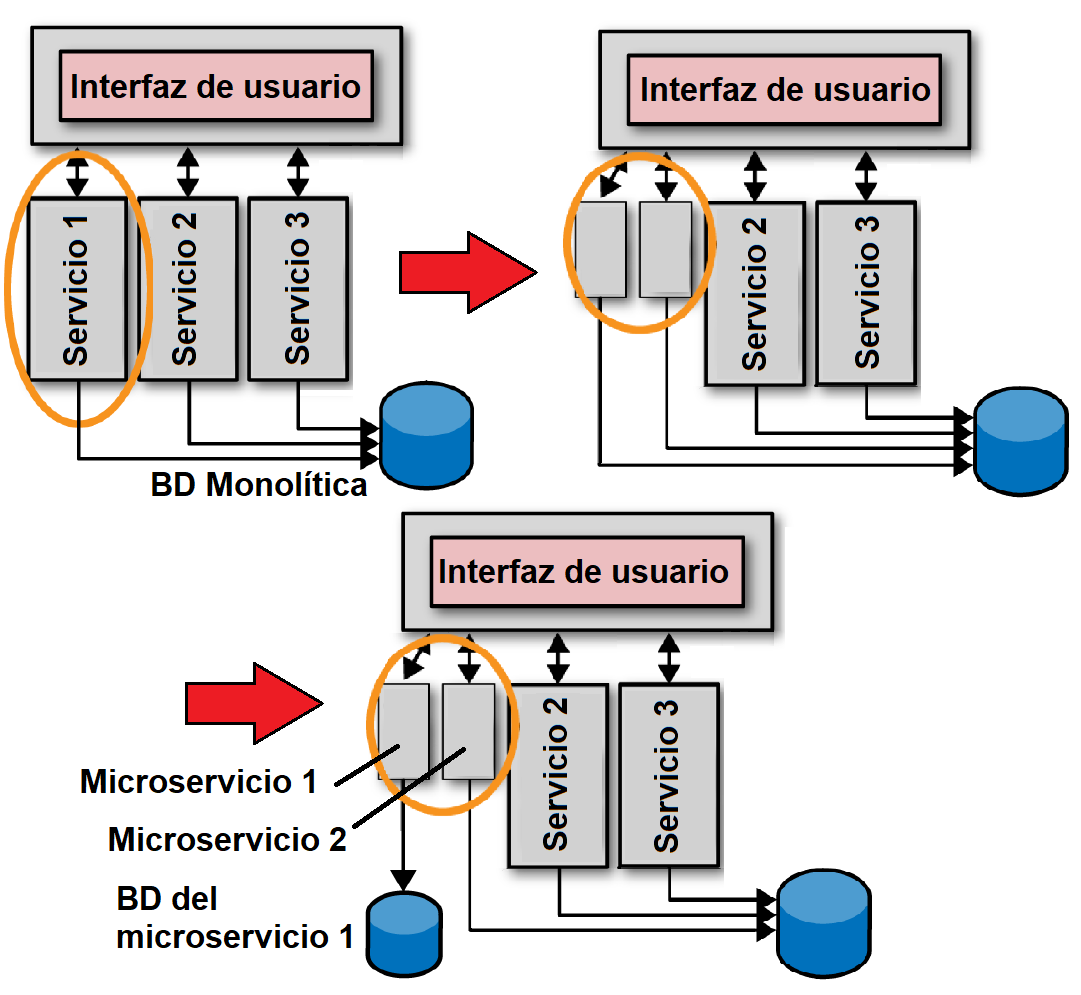
\includegraphics[scale=0.4]{refactoring}
\caption{Primero, se dividen los grandes servicios en microservicios. Una vez hecho esto, se migran sus datos. \cite{Richards2016}}
\end{figure}

Cuando sea necesario realizar un cambio por nuevos requisitos del negocio, estos se localizarán en un contexto bien delimitado porque existirá una correspondencia entre la estructura de la organización y los microservicios del sistema. Como consecuencia, el tiempo medio para realizar un cambio se verá reducido porque solo hará falta volver a desplegar una porción del sistema. Además, la comunicación entre microservicios se asemejará a la existente entre las entidades del negocio.

\subsection{La tarea del arquitecto de software}

El software ha de ser diseñado para ser flexible, adaptarse y evolucionar en función de los requisitos de los usuarios. En lugar de centrarse en diseñar un producto final perfecto, el arquitecto debe crear un entorno donde el sistema correcto pueda emerger creciendo progresivamente a medida que se descubren nuevos requisitos. Gracias a su modularidad, los microservicios son el entorno perfecto para que esto ocurra.

El arquitecto de software debe preocuparse más por como interaccionan los servicios entre ellos y no tanto en lo que ocurre dentro de sus límites. En organizaciones grandes, cada microservicio puede estar desarrollado por un equipo distinto y es el arquitecto quien debe hacer de puente entre ellos. \cite{Newman2015a}

Una de las ventajas de las arquitecturas basadas en microservicios es la \textbf{heterogeneidad tecnológica}: cada servicio puede ser desarrollado empleando una pila tecnológica distinta. No obstante, dejar plena libertad a cada equipo para elegir la tecnología del servicio que va a desarrollar puede traer problemas a la hora de integrarlo con el resto del sistema. El uso de contratos o establecer normas en aspectos clave como el protocolo de comunicación entre los servicios facilitará su consumo. Las decisiones de diseño de un servicio en particular pueden recaer en el equipo responsable. En este caso, el arquitecto solo juega un papel de supervisor y asesor para evitar que se pierda la imagen del sistema completo.

\section{Los microservicios en la fase de implementación}

La fase de implementación consiste en la creación de un sistema o componente software combinando técnicas de programación, verificación y depuración. Esta fase emplea la salida de la fase de diseño y sirve como entrada para la de pruebas. Los límites entre estas tres fases varían en función del proceso seguido. \cite{Bourque2014}

\subsection{Integración de microservicios}

La \textbf{integración} es la parte más relevante en los sistemas basados en microservicios. Hacerlo correctamente nos asegurará su autonomía y su despliegue de manera independiente.

Por un lado, la tecnología empleada para la comunicación entre servicios no debe restringir la tecnología empleada en estos. Por otro lado, los consumidores deberían de tener total libertad en la tecnología que emplean y consumir un servicio para ellos no debe ser complejo de implementar. Además, los consumidores no deben conocer detalles internos del servicio que consumen para garantizar que estén desacoplados. \cite{Newman2015a} Existen muchas técnicas para la integración entre las que destacan: 

\begin{itemize}

\item \textbf{RPC} (Remote Procedure Call):la llamada a procedimiento remoto es una técnica que permite ejecutar una llamada a un servicio como si de una llamada local se tratara. No es necesario que cliente y servidor empleen la misma pila tecnológica, aunque algunas tecnologías como Java RMI (Remote Method Invocation) sí lo requieren. 

El formato de los mensajes también varía de una tecnología a otra. SOAP (proviene del inglés Simple Object Access Protocol) emplea XML (también del inglés eXtensible Markup Language) mientras que por ejemplo Java RMI transmite mensajes binarios.

\item \textbf{REST} (Representational State Transfer): la transferencia de estado representacional es un estilo arquitectónico inspirado en la Web. Se basa en el concepto de recurso, un objeto que el servicio conoce y del que puede crear diferentes representaciones bajo demando. La representación del recurso está completamente desacoplada de como se almacena.

La arquitectura REST es ampliamente usada junto con HTTP (término que proviene del inglés Hypertext Transfer Protocol). Los verbos que se definen en HTTP actúan sobre recursos: por ejemplo, con el verbo GET se puede obtener una representación del recurso y con el POST crear uno nuevo.

\item \textbf{Integración basada en eventos}: en la integración basada en eventos, un servicio publica un evento cuando sucede algo relevante. Al evento se suscriben aquellos componentes que deben reaccionar al evento producido. Para hacer llegar los eventos a sus consumidores se debe mantener una nueva infraestructura, como puede ser una cola basada en mensajes.

\begin{figure}[h]
\centering
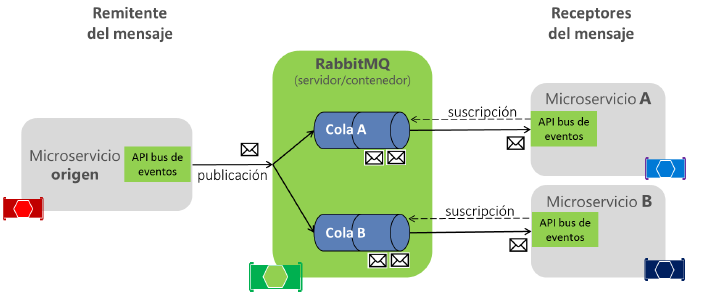
\includegraphics[scale=0.85]{rabbitmq}
\caption{Ejemplo de integración basada en eventos con un contenedor de RabbitMQ. \cite{DelaTorre2018}}
\end{figure}

Un bróker de mensajería es un patrón arquitectónico para la validación, la transformación y el enrutamiento de mensajes. RabbitMQ es un ejemplo de este patrón. En esta herramienta, el productor de un evento publica este a través de una API, donde será tramitado por el bróker para hacerlo llegar a todos los consumidores suscritos.
 
\end{itemize}

Tanto SOAP como REST emplean HTTP, aunque solo el segundo emplea los verbos definidos en HTTP. Existen pocas librerías para trabajar con SOAP, mientras que prácticamente cualquier lenguaje de programación contemporáneo cuenta con un cliente HTTP, con soporte para más o menos verbos. En cuanto a su rendimiento, REST es más eficiente en términos de latencia y ancho de banda consumido. \cite{Mulligan} REST es más recomendable que SOAP para enviar grandes volúmenes de datos por ser más compacto y permitir formatos como el JSON o el binario. Sin embargo, ni uno ni otro son recomendables para trabajar en redes con latencias bajas porque emplean HTTP. En este caso, es mejor emplear directamente protocolos como TCP o UDP. 

En cuanto al tercer tipo de integración, la integración basada en eventos fomenta la escalabilidad y resilencia de los servicios y reduce el acoplamiento entre ellos. No obstante, requiere aprovisionar nuevas infraestructuras y añade complejidad a la hora de razonar sobre el sistema por ser una comunicación asíncrona. Algunas buenas prácticas para afrontar su complejidad van desde el uso efectivo de sistemas de monitorización hasta el uso de identificadores de correlación para trazar las llamadas entre servicios. \cite{Newman2015a}

\subsection{Programación y persistencia políglotas}

%TODO Sustituir anteriormente por enlace.
Como hemos comentado anteriormente, diferentes microservicios se pueden desarrollar empleando diferentes tecnologías. La base de datos que contiene los datos del servicio o la arquitectura interna del microservicio también pueden adaptarse a los requisitos del mismo. \cite{DelaTorre2018} La \textbf{programación políglota} se fundamenta en que diferentes lenguajes de programación son más aptos para tratar problemas específicos. Es más productivo escoger el lenguaje adecuado para un servicio concreto que tratar de buscar un lenguaje que se ajuste a los requisitos de todos.

\begin{figure}[h]
\centering
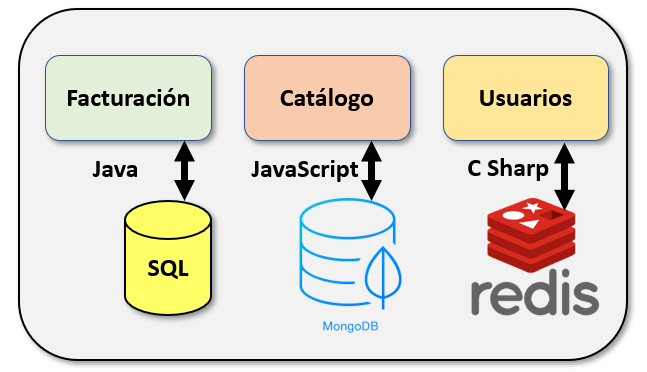
\includegraphics[scale=0.65]{poliglota}
\caption{Ejemplo de sistema políglota.}
\end{figure}

El término también se puede extrapolar a la persistencia. La \textbf{persistencia políglota} emplea diferentes tecnologías para la persistencia en función de los datos a almacenar y de cómo estos se van a manipular. Cada microservicio es dueño de sus datos y puede emplear una tecnología diferente. Las bases de datos relacionales no son la única opción y se deben considerar otras que escalen mejor si el servicio recibe muchas peticiones o se quiere hacer una explotación eficiente de los datos. \cite{Fowler2011}

En ambos casos, se debe hacer balance entre los beneficios que puede aportar un diseño políglota y sus costes asociados, por ejemplo, de aprendizaje.

\subsection{Microservicios en la interfaz de usuario}

\subsection{Ley de Conway}

\section{Los microservicios en la fase de pruebas}
% Art of unit testing
% Building microservices
% Simian army

Las pruebas de software consisten en la verificación dinámica de que un programa produce las salidas esperadas para un conjunto finito de casos de prueba. Las pruebas son dinámicas porque se verifica el programa en ejecución. Los casos de prueba son finitos porque el número posible de pruebas es infinito y estos se seleccionan en función de la prioridad y riesgo del código bajo pruebas. Además, se debe comprobar la salida obtenida con el resultado esperado para comprobar si esta es o no aceptable. \cite{Bourque2014}

\subsection{Pruebas unitarias}

Una \textbf{prueba unitaria} es una pieza de código que invoca al método o clase bajo prueba y que comprueba ciertas asunciones sobre su lógica. Se ejecuta de forma rápida y sencilla, está automatizado y es fácilmente mantenible. \cite{Osherove2014} En general, se prefiere tener un gran número de este tipo de pruebas por su rapidez, porque pueden ayudar a la refactorización del código y porque es donde mayor cantidad de defectos se suele capturar.

\begin{figure}[h]
\centering
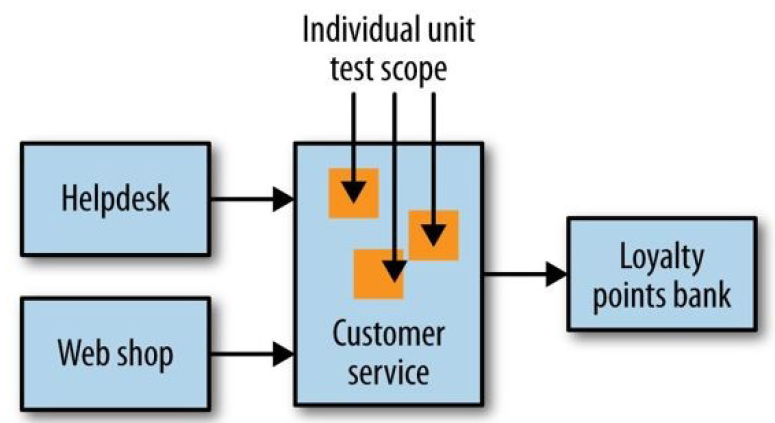
\includegraphics[scale=0.5]{Unit_Tests}
\caption{Diagrama de pruebas unitarias.}
\end{figure}

\subsection{Pruebas de servicios}

En las \textbf{pruebas de servicios} se verifica cada una de las funcionalidades que un servicio expone. Se pretende verificar el servicio de forma aislada y para ignorar las dependencias que el servicio bajo pruebas tiene sobre otros se reemplazan los servicios colaboradores por fakes.

Encajan dentro de las pruebas de integración, que se definen como la prueba como un conjunto de dos o más módulos de software que colaboran para evaluar un resultado esperado. \cite{Osherove2014} Este tipo de pruebas pueden ser igual de rápidas que las unitarias siempre que no se tengan que emplear un gran número de infraestructuras como bases de datos o colas.

\begin{figure}[h]
\centering
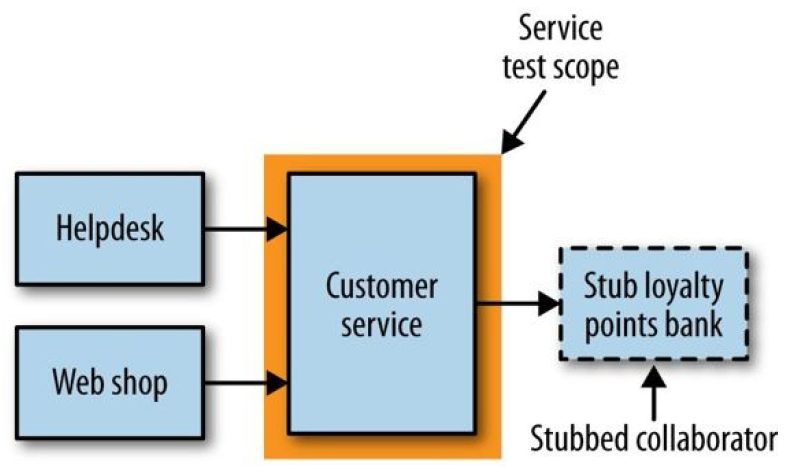
\includegraphics[scale=0.5]{Service_Tests}
\caption{Diagrama de pruebas de servicios.}
\end{figure}

\subsection{Pruebas de extremo a extremo}

Las \textbf{pruebas de extremo} a extremo son pruebas que se ejecutan sobre todo el sistema. Cubren gran parte de código, por lo que su correcta ejecución dan mucho grado de confianza. En su ejecución se levantan varios servicios diferentes.

Son pruebas frágiles: conforme el alcance de la prueba aumenta más son las partes sobre las que no se puede tener control. Estas partes pueden introducir fallos que no demuestran que la funcionalidad tenga un defecto y hacen la prueba menos determinista. Si la prueba falla continuamente, el equipo encargado puede llegar a asumir como normal está situación. Su tiempo de ejecución es mayor y en consecuencia, más tarde se detecta si un cambio ha introducido un defecto. \cite{Newman2015a}

\begin{figure}[h]
\centering
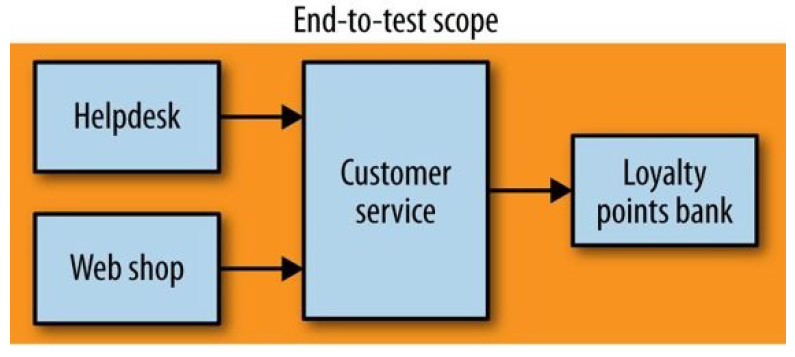
\includegraphics[scale=0.5]{End_To_End_Test}
\caption{Diagrama de pruebas de extremo a extremo.}
\end{figure}

\subsection{Balance de pruebas a realizar}

A medida que aumenta el alcance de las pruebas lo hace el nivel de confianza que las pruebas dan sobre la ausencia de defectos. Por otro lado, cuanto más arriba en la pirámide más tiempo tardará una prueba en implementarse y ejecutarse. Además, determinar el motivo de fallo de una prueba será más costoso cuanto mayor sean las líneas de código probadas. \cite{Cohn2010}

\begin{figure}[h]
\centering
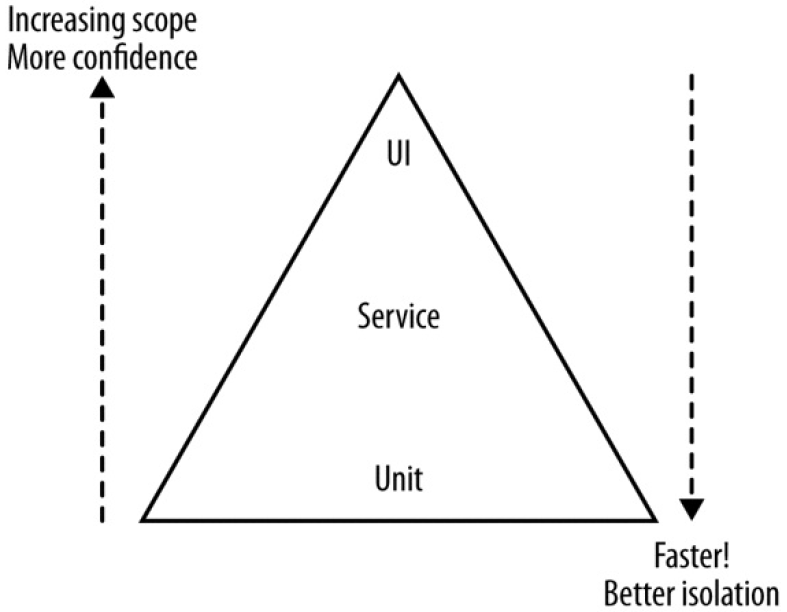
\includegraphics[scale=0.5]{Cohn_Pyramid}
\caption{Pirámide de pruebas diseñada por Mike Cohn. \cite{Cohn2010}}
\end{figure}

El número de pruebas que se aconseja tener de cada tipo aumenta conforme descendemos por la pirámide. El número de servicios que participan para ofrecer una funcionalidad al usuario puede ser muy alto y en una prueba no se deberían de levantar más de 3 o 4 servicios para no potenciar las desventajas que hemos mencionado. Por este motivo, las pruebas de extremo a extremo deben ser las mínimas posibles y se deben refactorizar en pruebas de servicios que empleen fakes siempre que se pueda.

\section{Los microservicios en la fase de despliegue}
% Docker
% Kubernetes
% Orquestadores (¿Moltó?)
% Azure y AWS
% CI/CD

El despliegue se define como la entrega de software (como un producto completo o como resultado de un incremento en un desarrollo incremental) al cliente para que este lo evalúe y devuelva retroalimentación al equipo de desarrollo. \cite{Pressman} Debido a la naturaleza incremental de la mayoría de procesos de desarrollo, esta es una actividad que se realiza numerosas ocasiones. 

En cada despliegue, se debe proveer del soporte necesario para el empleo de las nuevas características. Además, la retroalimentación recibida guiará el proceso de desarrollo hacia las siguientes modificaciones y funcionalidades que se deben realizar.

Los problemas que aparecen en una nueva versión del producto deben ser atendidos. Para garantizar que estos no ocurran, se deben hacer pruebas en cuantos más entornos posibles mejor.

\subsection{Integración y entrega continua}

La \textbf{integración continua} es una práctica en el desarrollo de software donde los miembros del equipo integran su trabajo de forma frecuente, normalmente a diario. Cada integración se verifica mediante compilaciones automatizadas que incluyen la ejecución de pruebas para detectar errores y conflictos en la integración. \cite{Fowler2006} El término tiene su origen como una de las doce prácticas de la metodología Extreme Programming (XP).

Durante este proceso se crean artefactos sobre los que se ejecutarán validaciones. Los artefactos construidos deben ser lo más parecidos a los que más tarde se despliegan en la versión de producción para asegurar que es el mismo artefacto sobre el que se han hecho las pruebas. Entre los beneficios de la integración continua encontramos:
 
\begin{itemize}

\item \textbf{Rápida retroalimentación}: los desarrolladores obtienen más rápido una respuesta sobre la calidad de sus cambios. Con este fin, la compilación ha de ser lo más rápido posible. Se pueden obtener mayores beneficios de la integración continua a través de las compilaciones por fases o build pipelines. En este tipo de compilaciones se separa por pasos el proceso. Los pasos de la pipeline pueden ser manuales, como las pruebas de aceptación de un usuario, o estar automatizados, como la ejecución de pruebas unitarias. La ventaja de hacer esto es que se obtiene una retroalimentación más rápida si se ejecutan de forma separada acciones rápidas de otras más pesadas. \cite{Fowler2006}

\item \textbf{Equipo sincronizado}: los integrantes de un equipo obtienen más rápido los cambios que otros han realizado y conocen en todo momento el estado de la compilación. Si esta falla, arreglarla es la prioridad número uno.

\item \textbf{Trazabilidad}: si el código está bajo control de versiones, en cualquier momento se puede volver a construir un artefacto de una versión concreta a partir del código que la origina. \cite{Newman2015a}

\end{itemize}

\begin{figure}[h]
\centering
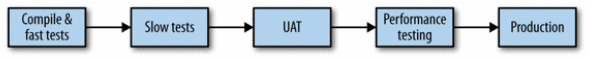
\includegraphics[scale=1]{pipeline}
\caption{Ejemplo de una pipeline. \cite{Newman2015a}}
\end{figure}

La \textbf{entrega continua} extiende la idea de la integración continua en cuanto a que cada cambio que ha superado la compilación puede ser candidata para ser desplegada en producción en cualquier momento. Sobre cada cambio se puede decidir si se publica o no a producción y hacerlo no cuesta más que pulsar un botón porque está todo el proceso de despliegue automatizado. La práctica de que cada cambio que se realiza y supera la pipeline es publicado automáticamente a producción se denomina \textbf{despliegue continuo}. \cite{Fowler2013}

\subsection{Virtualización y tecnología de contenedores}

Un \textbf{host} representa una unidad genérica de aislamiento, un sistema operativo donde se pueden instalar y ejecutar servicios. Si desplegamos directamente sobre máquinas físicas, entonces un host será el equivalente a una de ellas. Sin embargo, tener muchos hosts es costoso si cada uno consiste en una máquina diferente. \cite{Newman2015a}

La \textbf{virtualización} nos permite dividir una máquina en hosts separados, donde pueden ejecutarse servicios distintos. En la virtualización tradicional, cada una de las máquinas virtuales (MV) puede ejecutar su propio sistema operativo. Un recurso adicional es añadido entre la máquina física y las virtuales: el hipervisor. El hipervisor reparte recursos de la máquina física como la CPU o la RAM entre los distintos hosts virtualizados y permite al usuario la gestión de las máquinas virtuales contenidas.

El mayor inconveniente de las máquinas virtuales es que se puede dividir una máquina en muchas piezas como queramos porque la separación entre los hosts supone un coste. El hipervisor también consume recursos y cuantas más son las máquinas que debe gestionar, mayor será su consumo. Además, el tiempo de puesta en funcionamiento de una máquina virtual es de la magnitud de minutos, mientras que el arranque de un contenedor ronda los pocos segundos. \cite{Dua2014} Esto es muy importante en desarrollos que siguen las técnicas de integración continua donde se despliegan artefactos frecuentamente. 

Los \textbf{contenedores} son sistemas operativos ligeros que se ejecutan sobre una máquina con la que comparten el kernel. El número de contenedores que una máquina puede alojar es mayor que el número de máquinas virtuales debido a la naturaleza ligera de estos. \cite{Dua2014} Su uso de recursos es y tiempo de aprovisionamiento son menores al de una MV, lo que reduce el tiempo de retroalimentación sobre el funcionamiento de un servicio. Sin embargo, el grado de aislamiento de los contenedores no es perfecto ya que existen formas en las que se puede interferir en el funcionamiento de otro contenedor debido a problemas de diseño y bugs conocidos. \cite{Newman2015a}

\begin{figure}[h]
\centering
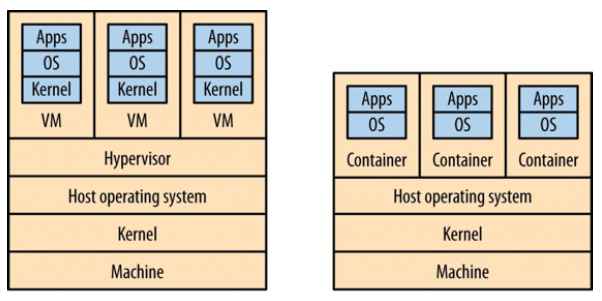
\includegraphics[scale=0.8]{containers_vms}
\caption{Comparación entre la virtualización y la contenerización. \cite{Newman2015a}}
\end{figure}

Ambas soluciones se pueden combinar para obtener las ventajas de ambas. Se puede obtener una máquina virtual de una plataforma como Amazon Web Services (AWS) que nos asegure características como la escalabilidad bajo demanda y sobre ella ejecutar diferentes servicios desplegados como contenedores.

\subsection{Docker}

Docker es una herramienta basada en contenedores Linux para la creación de artefactos que se pueden desplegar en cualquier entorno y se pueden distribuir y escalar bajo demanda. \cite{Matthias} Su funcionamiento es sencillo: en un fichero llamado \textbf{Dockerfile} se especifican las dependencias del servicio en distintos pasos y un comando que inicia el servicio. De la compilación del Dockerfile se origina una \textbf{imagen}, un paquete con todas las dependencias e información necesaria para crear un contenedor. Las imágenes permiten empaquetar un servicio para desplegarlo de forma confiable y reproducible tantas veces como se desee. \cite{DelaTorre2018}

La filosofía de Docker se centra en los contenedores desechables. Nada en el entorno donde se ejecuta la aplicación permanecerá ahí más allá de lo que viva la aplicación, por lo que no se delegará en entornos donde se encuentra casualmente una dependencia no especificada en la imagen. Docker promueve las arquitecturas sin estado (stateless) o que externalizan este a otras infraestructuras como bases de datos. Las aplicaciones así se hacen más portables, escalables y confiables. \cite{Matthias}

El proceso de desarrollo también se simplifica: en aproximaciones como la de microservicios, un equipo encargado de un servicio solo necesita la imagen de otro para integrarlo con el suyo y no necesita conocer detalles internos de este. Además, las tareas de construcción de la imagen, provisión de la configuración y despliegue pueden ser realizadas por diferentes personas, como se muestra en la figura. 

\begin{figure}[h]
\centering
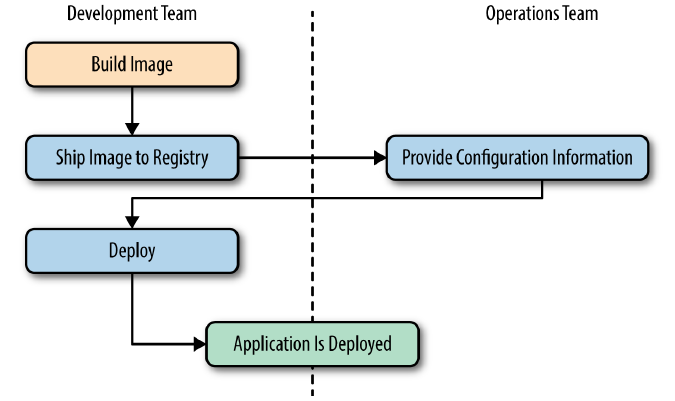
\includegraphics[scale=0.7]{docker_process}
\caption{Proceso de despliegue con Docker. \cite{Matthias}}
\end{figure}


Si se integra dentro del proceso de despliegue, cada cambio que pasa por una pipeline puede construir una nueva imagen Docker sobre la que se ejecutan pruebas de forma automatizada para después ser publicada a producción. De esta forma el equipo puede asegurarse de que el artefacto sobre el que se han ejecutado las pruebas es el mismo que se publica más tarde. 

\subsection{Kubernetes}

Kubernetes es una herramienta diseñada por Google para el despliegue y orquestación de aplicaciones en contenedores Docker de forma resilente. Cada una de las máquinas que aloja uno o más contenedores Docker se denomina \textbf{nodo}. La unidad más pequeña con la que trabaja Kubernetes no son los contenedores, sino los pods. Un \textbf{pod} es una colección de contendores y volúmenes agrupados juntos en un nodo. Los \textbf{volúmenes} son sistemas de archivos virtuales que se pueden emplear para comunicar entre ellos a los contenedores de un nodo. Kubernetes orquesta a nivel de los pods, por lo que dos contenedores en el mismo pod serán administrados igual. \cite{Rensin2015}

\begin{figure}[h]
\centering
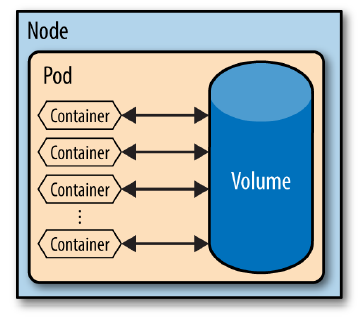
\includegraphics[scale=0.7]{kubernetes}
\caption{Un nodo de Kubernetes. \cite{Rensin2015}}
\end{figure}

Kubernetes se emplea principalmente para especificar el número de replicas que se desea tener simultánemanete de un pod. La herramienta es buena para asegurar la disponiblidad de un servicio, pero no garantizan la escalabilidad de este, que consistiría en modificar el número de replicas de un pod de forma dinámica en función de su demanda. Para este propósito se deben introducir balanceadores de carga como puntos de entrada al sistema. Estos balancenadores redirigirían cada petición al pod correspondiente y se encarguen de ajustar el número de replicas de un pod según una serie de reglas.

\section{Los microservicios en la fase de mantenimiento}
% You code, you run it -> Buscar documento "oficial"
% Monitorización
% Arquitectura evolutiva

Los productos software cambian y evolucionan. Una vez están desplegados en el entorno donde operan se dan situaciones en las que se detectan errores o los requisitos de los usuarios se ven modificados. Es una fase que debe comenzar de forma temprana para garantizar la mantenibilidad del sistema a desarrollar. \cite{Bourque2014}

El mantenimiento de software es la fase del desarrollo que más recursos consume, alrededor del 60\% o 70\% del coste de un proyecto. La mayoría del software que hoy se emplea tiene entre 10 y 15 años, tiempo en el cual ha sufrido muchas modificaciones hasta alcanzar un diseño pobre y difícil de mantener. Se puede definir el software mantenible como aquel que se diseña de forma modular, siguiendo patrones de diseño y estándares de calidad y que se documenta de tal forma que es explicativo por si mismo. \cite{Pressman} 

Gracias a su diseño modular, los microservicios son una arquitectura que se puede seguir para hacer más sencillo el mantenimiento de un sistema. Sin embargo, las consecuencias de elegir un estilo arquitectónico no son evidente hasta años más tarde de haber sido tomadas, por lo que hasta que no se vean sistemas maduros que empleen microservicios no se debe afirmar a ciencia cierta que garantizan estas características. \cite{Lewis2014}

\subsection{Reemplazamiento}

En la mayoría de empresas abundan los sistemas legados que nadie desea mantener. La \textbf{refactorización} de estos sistemas es imposible por su tamaño y riesgo. Si en lugar de haber empleado una arquitectura monolítica para su diseño se emplearan microservicios se observaría como los barreras para la refactorización no existen al poderse reescribir el microservicio al completo en pocos días.

Una regla que puede ser aplicada es establecer un tamaño para un microservicio tal que pueda ser completamente reescrito en 2 semanas. \cite{Newman2015a}

\subsection{You Build It, You Run It}

En muchas organizaciones, el desarrollo de sistemas se hace a través de proyectos: piezas de software que una vez desarrolladas se consideran completadas. En una aproximación basada en microservicios, cada equipo es responsable del ciclo de vida completo de un producto o servicio. Esto sigue la filosofía de Amazon: \textbf{"you build, you run it"}. \cite{Lewis2014}

No hay necesidad de distinguir entre quien construye un sistema y quien lo ejecuta y posteriormente mantiene. Esta filosofía aproxima a desarralloradores y clientes: los desarrolladores están en contacto directo con los clientes día tras día, lo que les proporciona retroalimentación para mejorar la calidad de sus servicios. Tampoco hay necesidad de contar en la organización con un equipo centrado en la infraestructura (IT). Contar con un equipo así distribuye la responsabilidad de hacer un servicio funcionar entre diferentes equipos y añade un sobreesfuerzo de coordinación y comunicación cuando un problema aparece. \cite{Vliet2011}

\subsection{Documentación}

Una de las ventajas de los microservicios es que acelara el proceso de desarrollo. Sin embargo, cuanto más rápido tratamos de implementar un servicio más probable es que tomemos atajos para poder desplegar antes una iteración del producto, lo que se traduce en un aumento de la \textbf{deuda técnica}. \cite{FowlerSusan}

En un equipo de desarrollo el conocimiento de cómo funciona un sistema se reparte entre los miembros que lo forman. Nadie es capaz de conocer completamente su funcionamiento y lo más probable es que cada desarrollador conozca mejor la parte donde más tiempo ha invertido. A la hora de realizar un cambio, el entendimiento de cómo funciona el sistema tiene que ser compartido por todos sus miembros para asegurar que el cambio a implementar es el correcto.

La documentación es una de las mejores maneras de solventar la deuda técnica y garantizar que el equipo de desarrollo conoce realmente cómo funciona un microservicio. Cabe recordar que cada microservicio puede seguir una arquitectura diferente o emplear una tecnología distinta. Debido a esto, se debe documentar de forma exhaustiva para facilitar la integración entre ellos y facilitar el traslado de personas de un equipo a otro.

\subsection{Monitorización}

Durante el mantenimiento se debe asegurar la disponibilidad de los microservicios. Las herramientas de monitorización son clave para garantizar los \textbf{acuerdos de nivel de un servicio} (SLA) y el estudio de errores cuando estos ocurren.

Con este propósito, se debe registrar toda aquella información relevante que ocurra. Los microservicios colaboran entre ellos para ofrecer funcionalidades concretas y recrear un sistema donde ha ocurrido un error puede ser complejo debido a que cada uno se versiona de forma independiente. Por ello, lo mejor es contar con toda la información necesaria registrada para determinar la causa del problema.

La información más útil se debe mostrar de forma gráfica a través de dashboards que reflejen el estado de salud de los servicios. Así, la informacón más consultada se puede visualizar de forma rápida y fácil de entender para ahorrar tiempo. No obstante, cuando un problema ocurre se debe hacer uso de alertas para atenderlo de forma prioritaria. Estas alertas han de ser accionadas automáticamente por métricas que superen un límite establecido, como puede ser el uso de recursos, o por la ocurrencia de excepeciones en el servicio. \cite{FowlerSusan}

\section{Comparación con otras arquitecturas}

\section{Crítica al estado del arte}
% Trabajos presentados en la ETSINF.

\section{Propuesta}
% Que mejora mi trabajo.

%%%%%%%%%%%%%%%%%%%%%%%%%%%%%%%%%%%%%%%%%%%%%%%%%%%%%%%%%%%%%%%%%%%%%%%%%%%%%%%
%                       ANALISIS DEL SISTEMA                                 %
%%%%%%%%%%%%%%%%%%%%%%%%%%%%%%%%%%%%%%%%%%%%%%%%%%%%%%%%%%%%%%%%%%%%%%%%%%%%%%%

\chapter{Análisis del sistema}

\section{Descripción del sistema}

Se desea desarrollar un sistema para la venta de productos electrónicos a través de dispositivos móviles. La aplicación móvil estará destinada solo a los clientes de una tienda, que deberán registrarse para usarla.

Los clientes podrán consultar los \textbf{productos} disponibles en la tienda junto con su precio, descripción y número de unidades en stock. Un \textbf{pedido} se define como un conjunto de productos que el cliente ha seleccionado junto con el número de unidades de cada uno. Mientras no se haya confirmado el pedido, se podrán añadir y eliminar productos al pedido en elaboración.

Todos los pedidos realizados por un cliente se mostrarán en un listado junto con el estado de los mismos. Para cada pedido, el cliente podrá generar una factura donde se listen los productos que lo componen y el precio total.

Una vez un cliente haya confirmado un pedido, este deberá ser aprobado por un empleado para ser entregado. Mientras que el empleado no lo apruebe, el pedido podrá ser cancelado. Además, cuando el pedido sea entregado físicamente al cliente, este deberá marcar el pedido como entregado.

Un cliente puede crear una \textbf{incidencia} si tiene algún problema con un pedido o quiere consultar una duda con los empleados de la tienda. Dentro de una incidencia, tanto el cliente como los empleados se comunicarán a través de \textbf{comentarios}. Cuando lo considere oportuno, el cliente podrá cerrar la incidencia creada, que podrá volver a consultar en cualquier momento.

\section{Casos de uso y modelo de dominio}

A continuación, vamos a listar los casos de uso de la aplicación móvil. El único usuario de la aplicación móvil es el cliente de la tienda, por lo que es el actor de todos los casos citados. Para cada caso de uso se va a proveer un identificador, un título y una descripción breve:

\begin{center}
\begin{tabular}{ | c | l | }
\hline
\textbf{ CU001 } & Iniciar sesión \\
\hline
\multicolumn{2}{ | p{14cm} | }
{
Para iniciar sesión, el usuario debe haberse registrado previamente en la aplicación. Para hacerlo debe proveer simplemente su correo electrónico y su contraseña.
} \\
\hline
\end{tabular}
\end{center}

\begin{center}
\begin{tabular}{ | c | l | }
\hline
\textbf{ CU002 } & Registrarse en la aplicación \\
\hline
\multicolumn{2}{ | p{14cm} | }
{
Cualquier persona que tenga la aplicación instalada en su dispositivo móvil puede registrarse como cliente. Para hacerlo, simplemente ha de proveer su nombre, su correo electrónico y una contraseña.
} \\
\hline
\end{tabular}
\end{center}

\begin{center}
\begin{tabular}{ | c | l | }
\hline
\textbf{ CU003 } & Listar los productos de la tienda \\
\hline
\multicolumn{2}{ | p{14cm} | }
{
El cliente puede consultar todos los productos disponibles en la tienda. Para cada producto se mostrará una imagen, el nombre del producto y su precio. El usuario podrá buscar un producto por su nombre y ordenar el listado por nombre y precio.
} \\
\hline
\end{tabular}
\end{center}

\begin{center}
\begin{tabular}{ | c | l | }
\hline
\textbf{ CU004 } & Visualizar un producto \\
\hline
\multicolumn{2}{ | p{14cm} | }
{
El cliente puede ver la descripción de un producto, su precio y número de unidades en stock. Cuando lo desee, el usuario puede seleccionarlo para comprarlo y crear así un nuevo pedido.
} \\
\hline
\end{tabular}
\end{center}

\begin{center}
\begin{tabular}{ | c | l | }
\hline
\textbf{ CU005 } & Crear un pedido \\
\hline
\multicolumn{2}{ | p{14cm} | }
{
El cliente puede crear un pedido y añadir en él productos. Para cada uno, debe especificar el número de unidades que desea. En cualquier momento puede eliminar cualquiera de los productos que componen el pedido. Cuando lo considere oportuno, el cliente ha de confirmar el pedido que está creando para que sea tramitado.
} \\
\hline
\end{tabular}
\end{center}

\begin{center}
\begin{tabular}{ | c | l | }
\hline
\textbf{ CU006 } & Cancelar un pedido \\
\hline
\multicolumn{2}{ | p{14cm} | }
{
Para los pedidos confirmados, mientras estos no hayan sido gestionados por un empleado para su entrega, el pedido se podrá cancelar.
} \\
\hline
\end{tabular}
\end{center}

\begin{center}
\begin{tabular}{ | c | l | }
\hline
\textbf{ CU007 } & Generar factura de un pedido \\
\hline
\multicolumn{2}{ | p{14cm} | }
{
El cliente podrá generar una factura para cualquiera de sus pedidos. La factura se generará en formato PDF e incluirá la siguiente información: los datos del cliente, el listado de todos los productos que componen el pedido junto con su precio unitario y el precio total del pedido antes y después de aplicar el IVA.
} \\
\hline
\end{tabular}
\end{center}

\begin{center}
\begin{tabular}{ | c | l | }
\hline
\textbf{ CU008 } & Marcar un pedido como recibido \\
\hline
\multicolumn{2}{ | p{14cm} | }
{
Cuando un pedido se entregue físicamente a un cliente, este deberá marcar a través de la aplicación el pedido como recibido.
} \\
\hline
\end{tabular}
\end{center}

\begin{center}
\begin{tabular}{ | c | l | }
\hline
\textbf{ CU009 } & Listar los pedidos del cliente \\
\hline
\multicolumn{2}{ | p{14cm} | }
{
Todos los pedidos que ha realizado un cliente se podrán listar en cualquier momento, mostrando la fecha en que se realizó y su estado actual. Los pedidos aparecen ordenados por la fecha en la que se realizaron. El listado se puede filtrar por el estado de los pedidos. Los posibles estados de un pedido son: CONFIRMADO, PROGRAMADO, RECIBIDO y CANCELADO.
} \\
\hline
\end{tabular}
\end{center}

\begin{center}
\begin{tabular}{ | c | l | }
\hline
\textbf{ CU010 } & Crear una incidencia \\
\hline
\multicolumn{2}{ | p{14cm} | }
{
Un cliente puede crear una incidencia si tiene algún problema con un pedido o quiere consultar una duda con los empleados de la tienda. Para hacerlo, ha de proveer un título que describa el problema o consulta.
} \\
\hline
\end{tabular}
\end{center}

\begin{center}
\begin{tabular}{ | c | l | }
\hline
\textbf{ CU011 } & Añadir un comentario en una incidencia \\
\hline
\multicolumn{2}{ | p{14cm} | }
{
En el contexto de una incidencia, los clientes podrán comunicarse a través de comentarios con los empleados de la tienda. En la incidencia se verán los comentarios tanto de los empleados como del cliente ordenados cronológicamente. Para cada comentario se mostrará el nombre del autor, la fecha en la que lo escribió y el contenido del mismo.
} \\
\hline
\end{tabular}
\end{center}

\begin{center}
\begin{tabular}{ | c | l | }
\hline
\textbf{ CU012 } & Cerrar una incidencia \\
\hline
\multicolumn{2}{ | p{14cm} | }
{
Solo el cliente puede cerrar una incidencia que haya abierto. Cuando lo haga, el cliente podrá seguir accediendo a ella pero ya no podrá añadir nuevos comentarios. Tampoco le estará permitido volver a abrirla.
} \\
\hline
\end{tabular}
\end{center}

\begin{center}
\begin{tabular}{ | c | l | }
\hline
\textbf{ CU013 } & Listar las incidencias del cliente \\
\hline
\multicolumn{2}{ | p{14cm} | }
{
Se pueden consultar todas las incidencias creadas por el cliente en un listado donde se mostrará tanto la fecha en la que se crearon como su estado actual. El listado aparecerá ordenado por la fecha de creación de las incidencias y se podrá filtrar por el estado de las mismas. Los posibles estados de las incidencias son: ABIERTA y CERRADA.
} \\
\hline
\end{tabular}
\end{center}

\section{Plan de trabajo}

%%%%%%%%%%%%%%%%%%%%%%%%%%%%%%%%%%%%%%%%%%%%%%%%%%%%%%%%%%%%%%%%%%%%%%%%%%%%%%%
%                       MONOLITICA
%
%%%%%%%%%%%%%%%%%%%%%%%%%%%%%%%%%%%%%%%%%%%%%%%%%%%%%%%%%%%%%%%%%%%%%%%%%%%%%%%

\chapter{Diseño e implementación de la solución monolítica}

\section{Diseño de la solución}

\section{Tecnología utilizada}

\section{Interfaz de usuario}

\section{Pruebas}

%%%%%%%%%%%%%%%%%%%%%%%%%%%%%%%%%%%%%%%%%%%%%%%%%%%%%%%%%%%%%%%%%%%%%%%%%%%%%%%
%                       MICROSERVICIOS
%
%%%%%%%%%%%%%%%%%%%%%%%%%%%%%%%%%%%%%%%%%%%%%%%%%%%%%%%%%%%%%%%%%%%%%%%%%%%%%%%

\chapter{Diseño e implementación de la solución basada en microservicios}

\section{Diseño de la solución}

\section{Diferencias respecto a la solución monolítica}

\section{Versionado de servicios y creación de paquetes NuGet}

\section{Adaptación de la interfaz de usuario}

\section{Adaptación de las pruebas}

\section{Despliegue}

%%%%%%%%%%%%%%%%%%%%%%%%%%%%%%%%%%%%%%%%%%%%%%%%%%%%%%%%%%%%%%%%%%%%%%%%%%%%%%%
%                       EVALUACIÓN
%
%%%%%%%%%%%%%%%%%%%%%%%%%%%%%%%%%%%%%%%%%%%%%%%%%%%%%%%%%%%%%%%%%%%%%%%%%%%%%%%

\chapter{Evaluación de las soluciones}

\section{Mantenimiento}

\subsection{Mantenimiento correctivo}

\subsection{Añadir una relación entre diferentes servicios}

\subsection{Migración de la infraestructura}

\section{Escalabilidad}

\section{Tolerancia a fallos}

%%%%%%%%%%%%%%%%%%%%%%%%%%%%%%%%%%%%%%%%%%%%%%%%%%%%%%%%%%%%%%%%%%%%%%%%%%%%%%%
%                      CONCLUSIONES                                 %
%%%%%%%%%%%%%%%%%%%%%%%%%%%%%%%%%%%%%%%%%%%%%%%%%%%%%%%%%%%%%%%%%%%%%%%%%%%%%%%

\chapter{Conclusiones}

%%%%%%%%%%%%%%%%%%%%%%%%%%%%%%%%%%%%%%%%%%%%%%%%%%%%%%%%%%%%%%%%%%%%%%%%%%%%%%%
%                     BIBLIOGRAFIA                                 %
%%%%%%%%%%%%%%%%%%%%%%%%%%%%%%%%%%%%%%%%%%%%%%%%%%%%%%%%%%%%%%%%%%%%%%%%%%%%%%%

\bibliography{Bibliografia/library}



%%%%%%%%%%%%%%%%%%%%%%%%%%%%%%%%%%%%%%%%%%%%%%%%%%%%%%%%%%%%%%%%%%%%%%%%%%%%%%%
%                           APENDICES  (Si HAY!)                           %
%%%%%%%%%%%%%%%%%%%%%%%%%%%%%%%%%%%%%%%%%%%%%%%%%%%%%%%%%%%%%%%%%%%%%%%%%%%%%%%

\APPENDIX

%%%%%%%%%%%%%%%%%%%%%%%%%%%%%%%%%%%%%%%%%%%%%%%%%%%%%%%%%%%%%%%%%%%%%%%%%%%%%%%
%                      VENTAJAS E INCONVENIENTES   
%
%%%%%%%%%%%%%%%%%%%%%%%%%%%%%%%%%%%%%%%%%%%%%%%%%%%%%%%%%%%%%%%%%%%%%%%%%%%%%%%

\chapter{Ventajas e inconvenientes del desarrollo basado en microservicios}


%%%%%%%%%%%%%%%%%%%%%%%%%%%%%%%%%%%%%%%%%%%%%%%%%%%%%%%%%%%%%%%%%%%%%%%%%%%%%%%
%                      NAVEGACIÓN   
%
%%%%%%%%%%%%%%%%%%%%%%%%%%%%%%%%%%%%%%%%%%%%%%%%%%%%%%%%%%%%%%%%%%%%%%%%%%%%%%%

\chapter{Modelo de navegación de la aplicación móvil}

%%%%%%%%%%%%%%%%%%%%%%%%%%%%%%%%%%%%%%%%%%%%%%%%%%%%%%%%%%%%%%%%%%%%%%%%%%%%%%%
%                      DESPLIEGUE  
%
%%%%%%%%%%%%%%%%%%%%%%%%%%%%%%%%%%%%%%%%%%%%%%%%%%%%%%%%%%%%%%%%%%%%%%%%%%%%%%%
\chapter{Despliegue del sistema basado en microservicios}

\section{Ejecución de un contenedor con Docker}

\subsection{Archivo Docker Compose}

\section{Introducción a Azure Kubernetes Service (AKS)}

\section{Depuración de contenedores a través de Azure}

%%%%%%%%%%%%%%%%%%%%%%%%%%%%%%%%%%%%%%%%%%%%%%%%%%%%%%%%%%%%%%%%%%%%%%%%%%%%%%%
%                      CREACIÓN DE CLIENTES CON NSWAG  
%
%%%%%%%%%%%%%%%%%%%%%%%%%%%%%%%%%%%%%%%%%%%%%%%%%%%%%%%%%%%%%%%%%%%%%%%%%%%%%%%

\chapter{Creación de clientes con NSwag}


\end{document}
